\documentclass[fr]{../../../eplsummary}

\usepackage{graphicx}

\hypertitle[']{\'Economie de l'entreprise}{4}{FSAB}{1803}
{Nicolas Cognaux\and Beno\^it Legat}
{Jean-Pierre Hansen et Julien Hendrickx}

\newcommand{\elasticity}{\varepsilon}
\newcommand{\pcompt}{\pi}
\newcommand{\ppur}{\pi_{\mathrm{pur}}}
\newcommand{\surplus}{s}
\newcommand{\surpluscons}{{S_c}}
\newcommand{\surplusprod}{S_p}
\newcommand{\surpluscoll}{S}

\newcommand{\Lagr}{\mathcal{L}}


\section{Le marché de concurrence parfaite}
\paragraph{Marché}
Un marché est un groupe de consommateurs et de producteurs
qui font des transactions d'une certaine quantité $q$ à un prix $p$.

Dans un marché, pour chaque quantité $q$, les producteurs ont un prix
minimum auquel ils veulent bien vendre qu'on appelle l'offre $O(q)$
et les consommateurs ont un prix
maximum auquel ils veulent bien acheter qu'on appelle demande $D(q)$.

L'offre est croissante et la demande est décroissante.
Du coup, le produit va être vendu tant que $O(q) \leq D(q)$.
On peut donc déterminer la quantité échangée $q^*$ par l'équation
$O(q^*) = D(q^*)$ et le prix $p^*$ sera alors $p^* = O(q^*) = D(q^*)$.

%On voit que le marché s'auto régule,
%on appelle ça le principe de la ``Main Invisible''.
% La main invisible c'est plus que la maximisation du profit
% indivisuel mène à l'optimum collectif...

\subsection{Hypothèse de concurrence parfaite}
\begin{description}
  \item[Atomicité] de l'offre et de la demande.
    Personne ne peut influencer le prix et
    les producteurs ne peuvent pas faire de coalition pour pouvoir le faire.
  \item[Homogénéité] du produit.
    Les producteurs ne peuvent pas différencier leurs produits des autres.
  \item[Transparence] du marché.
    Tout le monde connait tous les prix et quantités sur tous les marchés
    à tout instant.
  \item[Mobilité parfaite]
    Il y a une libre entrée/sortie du marché.
\end{description}

\subsection{Le consommateur}
Le consommateur a une utilité $u(q)$ qui donne le prix qu'il est prêt à payer
pour obtenir une quantité $q$ d'un bien.
Cette fonction est normalement croissante, sinon, ça signifiera qu'une unité
d'un bien a une utilité négative.
L'utilité de la $q$\ieme{} unité d'un bien est $u'(q)$, on
parle de disposition marginale à payer (autrement dit, de disposition
à payer pour une unité supplémentaire).
Cette fonction est souvent décroissante, c'est la satiété.

Seulement, le prix $p$ d'un bien sur un marché est lui constant.
Il ne change pas si c'est le premier achat d'un consommateur ou si
c'est le second.

Si le prix est $p$, le consommateur achètera le bien tant que
$u'(q) > p$, c'est à dire jusqu'à ce que $u'(q) = p$.

Il aura alors un surplus, qui est l'utilité totale qu'il avait
de la quantité $q$ moins ce qu'il a du payer
\[ \surplus(q) = u(q) - pq. \]
Si on ne connait que $u'(q)$, cette relation devient simplement
\begin{equation}
  \label{eq:surplus_1cons}
  \surplus(p, q) = \int_0^q u'(\tilde{q})\dif \tilde{q} - pq.
\end{equation}

Le surplus d'un consommateur représente également la ``perte'' qu'il
subirait si on lui enlevait la possibilité d'acheter toutes
les quantités au même prix $p$.

On remarque qu'en essayant de maximiser son surplus $\max_q u(q) - pq$,
il obtient $u'(q) = p$ ce qui est bien ce qu'on vient de prédire.
Ce comportement de consommateur est le price taker.
C'est son comportement en concurrence parfaite.

$p = u'(q)$ définit également la courbe de demande individuelle
du consommateur. La courbe de demande globale se définit alors
comme la ``somme horizontale'' des courbes de demandes individuelles.

\subsection{Le producteur}
Le producteur lui n'a pas d'utilité, il a un coût de production.
Bien évidemment, son coût n'est pas le même pour produire sa première unité
que pour produire sa 42\ieme{}.
Si c'est de plus en plus cher,
c'est à dire que $C_M$ est croissant,
on parle de rendement d'échelle \emph{décroissant}.
Si c'est de moins en moins cher,
c'est à dire que $C_M$ est décroissant,
on parle de rendement d'échelle \emph{croissant}.
C'est le cas des serveurs.
Le coût moyen d'un serveur est plus faible lorsqu'on en a beaucoup que
lorsqu'on en a peu.
C'est pour ça qu'on a pas tous un serveur chez soi mais qu'on loue
des serveurs à des entreprises qui en ont beaucoup.

En pratique, on regarde si le coût est convexe,
c'est à dire si sa dérivée seconde est positive.
Si c'est le cas, le rendement d'échelle est \emph{décroissant}.
Si par contre elle est concave, le rendement d'échelle est \emph{croissant}.

\begin{description}
  \item[Coût]
    Le coût de produire $q$ unité est appelé \emph{coût} et est noté $C(q)$.
    Le coût est constitué d'un coût fixe qu'on note $C_F$ qui ne dépend
    pas de $q$ et qui doit être payé quoi qu'il arrive,
    même si $q = 0$, et d'un coût
    variable $C_V(q)$ qui dépend de $q$.
    Le coût fixe est un coût à payer lorsqu'on commence à produire
    et ne dépend pas du nombre d'unité qu'on produit. On a
    \[ C(q) = C_F + C_V(q). \]
  \item[Coût moyen]
    Le coût moyen est noté $C_M$, c'est simplement
    \[ C_M(q) = \frac{C(q)}{q}. \]
    On a aussi le coût fixe moyen
    \[ C_{FM}(q) = \frac{C_F}{q} \]
    et le coût variable moyen
    \[ C_{VM}(q) = \frac{C_V}{q}. \]
  \item[Coût marginal]
    Le coût marginal est noté $C_m$, c'est le coût de la $q$\ieme{} unité
    \[ C_m(q) = \fdif{C(q)}{q}. \]
    Ça n'a pas de sens de parler de coût fixe marginal car il serait nul
    ni de coût variable marginal car c'est le même que le coût marginal.
\end{description}

Un producteur en concurrence parfaite se comportent en \emph{price taker}.
C'est à dire qu'il regarde le prix actuel et qu'il offre jusqu'à
ce que ça lui coûte plus cher de produire une unité de plus que ce que
ça leur fait gagner.

Il ne prend pas l'équation du prix en fonction de la quantité
qu'il produit $p = D(q)$ pour pouvoir trouver $\fpart{p}{q}$,
il considère $p$ constant et donc $\fpart{p}{q} = 0$.
En effet, c'est impossible en concurrence parfaite de trouver
l'équation du prix en fonction de sa quantité.
%TODO qui fait ça ?

Il optimise donc son profit comptable
\[ \pcompt(q) = pq - C(q). \]
ce qui donne $p^* = C_m(q^*)$.

Seulement, le producteur ne produira pas si c'est plus avantageux de
ne rien faire.
En effet, ce n'est pas parce qu'on a pris $q^*$ tel que $\pi'(q^*) = 0$ qu'on
est à un maximum de $\pi(q)$.
S'il ne fait rien, il a un profit de
$\pcompt(0) = p \cdot 0 - C_F - C_V(0) = -C_F$.
Il produira donc $q^*$ si
\[ \pcompt(q^*) = p^* \cdot q^* - C_F - C_V(q^*) \geq -C_F = \pcompt(0) \]
et il produira 0 sinon.

On peut donc juste affirmer que si $q^* > 0$, alors $p^* = C_m(q^*)$.

\subsubsection{Profit comptable et profit économique}
Le profit comptable $\pcompt$ est tout simplement le profit auquel on s'attend.
Ce que l'entreprise gagne $pq$ moins ce que ça lui a coûté.

Le profit économique $\ppur$ est son profit comptable moins le meilleur
profit comptable qu'elle peut avoir autre part.
Donc par exemple, si Samsung, qui travaille dans le hardware avec
$\pcompt = 100$, pouvait obtenir $\pcompt = 50$ en travaillant dans le software ou
$\pcompt = 120$ en travaillant dans l'agriculture, son profit économique serait
$\ppur = -20$. Samsung devrait donc se lancer dans l'agriculture.

\subsubsection{Économies ou déséconomies externes}
Il se peut que le coût d'un producteur 1 dépende non seulement de la quantité
qu'il produit mais aussi de la quantité qu'un producteur 2 produit.
Par exemple si le producteur 1 utilise un fleuve pour refroidir ses
machines et qu'en amont, le producteur 2 l'utilise aussi pour refroidir ses machines.
Plus le producteur 2 l'utilise, plus le fleuve se réchauffera et plus le
coût du producteur 1 sera élevé.
On doit donc écrire
\begin{align*}
  C_1 & = C_1(q_1, q_2) & C_2 & = C_2(q_1,q_2).
\end{align*}

Si $\fpart{C_1}{q_2} < 0$, on dit que $C_1$ subit une économie externe.
Sinon, si $\fpart{C_1}{q_2} > 0$, on dit qu'il subit une déséconomie
externe.

Le problème c'est qu'en laissant les producteurs maximiser leur profit
et donc faire $p(q_1, q_2) = \fpart{C_i(q_1, q_2)}{q_i}$
(toujours en price-taker, bien entendu),
on arrive plus à un optimum collectif
(mais rien ne dit qu'on est pas à un optimum de Pareto).
Celui qui subit une déséconomie externe va perdre par rapport à l'optimum
collectif et l'autre va gagner.
Pour avoir l'optimum collectif,
il faut optimiser $\pcompt_1(q_1, q_2) + \pcompt_2(q_1, q_2)$
en utilisant le gradient et
non optimiser $\pcompt_1$ et $\pcompt_2$ séparément.

\subsubsection{Répartition de production}
Supposons qu'une firme ait plusieurs usines et
qu'elle doive répartir sa production sur ces différentes usines.
Chacune des usines a une fonction de coût $C_i(q_i)$ et elles peuvent
avoir une limite $\bar{q_i}$
(si elles en ont pas, on peut dire que $\bar{q_i} = \infty$)
qui impose que
\[ 0 \leq q_i \leq \bar{q_i}. \]

Si la répartition $q = q_1 + q_2 + \ldots + q_n$ minimise le coût de
production de $q$, alors il existe $C_m^*$ tel que
\begin{itemize}
  \item Si $0 < q_i < \bar{q_i}$, alors $C_{i,m}(q_i) = C_m^*$;
  \item Si $q_i = 0$, alors $C_{i,m}(q_i) \geq C_m^*$;
  \item Si $q_i = \bar{q_i}$, alors $C_{i,m}(q_i) \leq C_m^*$.
\end{itemize}

Pour la deuxième condition,
il faut faire attention au cas où le coût fixe
n'est pas obligatoire ($C_i(0) = 0$),
il faut alors considérer que $C_{i,m}(0)=\infty$,
la deuxième condition est donc toujours vérifiée pour $i$.

Si le rendement est croissant,
on a naturellement intérêt à moins répartir la production et à
tout produire dans l'usine où $C_{i,m}$ est le plus bas.

\subsection{Le collectif}
Le collectif, c'est les consommateurs et les producteurs rassemblés.
%Le surplus collectif $\surpluscoll$ est donné à l'équilibre $(p^*, q^*)$

Le surplus des consommateurs, c'est la somme du surplus de chaque consommateur
$\surpluscons(q) \eqdef \sum_i s_i(q)$.
Si on note le prix $p(q) \eqdef \sum_i u_i'(q)$, on a, par \eqref{eq:surplus_1cons},
\[ \surpluscons(q) = \int_0^{q}p(\tilde{q}) \dif \tilde{q} - p(q) q. \]

Le surplus des producteurs, c'est la somme du profit comptable de chaque
producteur
$\surplusprod(q) \eqdef \sum_i \pcompt_i(q_i)$.
On a donc (en prenant, la quantité totale vendue, $q = \sum_i q_i$)
\[ \surplusprod(q_1, \ldots, q_n) = p(q)q -
\sum_i \int_0^{q_i} {C_m}_i(\tilde{q}) \dif \tilde{q}. \]

Le surplus collectif est simplement
$\surpluscoll(q_1, \ldots, q_n)
\eqdef \surpluscons(q) + \surplusprod(q_1, \ldots, q_n)$.
D'où
\[ \surpluscoll(q_1, \ldots, q_n) =
  \int_0^{q}p(\tilde{q}) \dif \tilde{q}
- \sum_i \int_0^{q_i} {C_m}_i(\tilde{q}) \dif \tilde{q}. \]

On remarque qu'en voulant optimiser le surplus collectif
(en prenant $\grad \surpluscoll(q_1, \ldots, q_n) = 0$),
on arrive à $p(q) = {C_m}_i(q_i)$ $\forall i$.
On a appelle ça l'\emph{optimum collectif}.

Seulement, en laissant les producteurs agir en price taker
(ce qu'ils feront car on est en concurrence parfaite),
on aura des $q_i$ tels que $p(q) = {C_m}_i(q_i)$.
On comprend ici mieux ce que veut dire agir en price taker.
Effet, on pourrait se demander pourquoi, pour optimiser
$p(q)q_i - {C}_i(q_i)$, il considère que $\fpart{p(q)}{q_i} = 0$.
Pour expliquer cela,
il faut soit considérer que le producteur $i$ ne connaît pas la fonction $p(q)$
mais ne connaît que la valeur de $p$ actuelle, soit considérer qu'il
ne s'attend pas à ce que $\dif q = \dif q_i$, c'est à dire que s'il modifie
$q_i$, il s'attend de toute façon à ce qu'il y ait pleins d'autre changements
$\dif q_j$ et qu'il ne peut donc absolument pas prévoir $\dif q$ en fonction
de $\dif q_i$. Il considère alors $p$ constant en fonction de $q_i$,
faute de mieux.
%TODO cfr autres ? Cad ?

On remarque que l'équilibre naturel de concurrence parfaite mène à
un optimum collectif.
La maximisation du profit individuel mène donc à un optimum collectif.
C'est ce qu'Adam Smith appelle la ``Main Invisible''.

\subsubsection{Optimum de Pareto}
Soient $k$ marchés, $m$ consommateurs et $n$ producteurs.
Chaque marché a un prix $p_j$ et chaque producteur ou consommateur $i$
échange une quantité $q_{i;j}$ sur le marché $j$.

Chaque producteur a donc un profit économique
\[ \pcompt_i(q_{i;1},\ldots,q_{i;k}) = -C(q_i) + \sum_{j=1}^k p_jq_{i,j} \]
et chaque consommateur un surplus
\[ \surplus_i(q_{i;1},\ldots,q_{i;k}) = u(q_i) - \sum_{j=1}^k p_jq_{i,j} \]

S'il n'existe aucun autre état ($p_j$ et $q_{i;j}$)
tel qu'il y ait un $i$ tel que $\pcompt_i$ ou $\surplus_i$ augmente et
qu'\emph{aucun} $i$ tel que $\pcompt_i$ ou $\surplus_i$ diminue existe,
cet état est appelé \textbf{Pareto optimal}.
Il faut donc qu'on ne puisse pas augmenter la satisfaction d'un individu
sans en faire perdre à un autre.
Un état Pareto optimal n'est donc pas nécessairement équitable.

De plus,
la définition ne mentionne pas que l'augmentation de la satisfaction doive
se faire en respectant la loi du marché,
un prix unique etc...
Ni même que cette situation soit stable.
Quand on dit ``augmenter la satisfaction'',
cela veut dire ``serait-il possible à un observateur/décideur
externe de créer une situation en décidant du comportement de chacun,
qui aurait pour résultat d'améliorer la satisfaction
de quelqu'un sans diminuer celle d'un autre''.

Un optimum collectif est Pareto optimal mais tout état Pareto optimal
n'est pas spécialement un optimum collectif.

Quelques grands philosophes utilitaristes se sont penchés sur la question.
\begin{figure}
  \centering
  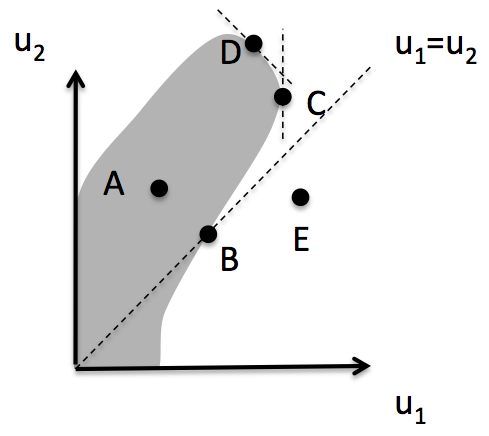
\includegraphics{pareto.png}
  \caption{Différents choix d'états}
  \label{fig:pareto}
\end{figure}
Sur la \figuref{pareto},
on a un graphe avec comme axes $u_1,u_2$ qui sont les
utilités de deux consommateurs.
Il y a une zone grisée donnant les états possibles.
E n'est donc pas un état possible.
Les points qui sont à l'intérieur des états possibles mais pas sur
la frontière ne peuvent pas être pareto optimaux.
Le point A est donc un état possible mais pas un état Pareto optimal.

Tous les points frontières ne sont pas spécialement Pareto optimaux,
pour être un point frontière Pareto optimal,
il faut que si on dessine des axes parallèles aux axes de départ
centrés en ce point, le premier quadrant ne contienne aucun état possible.
On voit bien ici pourquoi aucun point intérieur n'est Pareto optimal.
Ça nous permet aussi de dire que les seuls points Pareto optimaux sont
D et C.

\begin{description}
  \item[Égalitarisme]
    L'égalitarisme consiste à prendre l'intersection du contour
    avec la droite $u_1 = u_2$ ce qui donne le point B
    de la figure~\ref{fig:pareto}.
    On veut que les utilités soient exactement égales.
    Malheureusement on est parfois loin de maximiser la somme des
    utilités.
  \item[Bentham]
    Pour Bentham justement le plus important, c'est de maximiser la somme
    des utilités.
    Il prend donc la droite $u_1 + u_2 = s$ et fait augmenter $s$ jusqu'à
    ce qu'elle n'ait plus d'intersection avec le contour.
    Ça donne le point D de la figure~\ref{fig:pareto}.

    On voit que tous les états choisis par Bentham sont
    \emph{Pareto optimaux}.
    En effet, si le premier quadrant n'était pas vide, on pourrait
    encore augmenter $s$.
  \item[Rawls]
    Rawls essaie de faire un compromis entre les deux.
    Il essaie d'être plus égalitaire mais permet tout de même une disparité.

    Il se déplace donc sur la droite de l'égalitarisme $u_1 = u_2$
    et puis, pour un certain point de la droite $u_1 = u_2 = s$,
    on essaie de revenir sur le contour en augmentant $u_1$ seul ou en
    augmenant $u_2$ seul, c'est à dire qu'on trace les demi-droites
    $(u_1,s)$ avec $u_1 \geq s$ et $(s,u_2)$ avec $u_2 \geq s$.

    Pour essayer de maximiser la somme des utilités en minimisant la
    disparité, il va donc prendre le $s$ le plus grand tel que les demi-droites
    aient une intersection avec le contour.
    Ça nous donne le point C de la figure~\ref{fig:pareto}

    On peut aussi voir ça comme une maximisation de l'utilité minimale.
    En effet, si pour chaque point, on diminue les $u_i$ plus grands
    que les autres jusqu'à arriver à la droite $u_1 = u_2 = s$ et maximiser
    ce $s$ auquel on arrive, ça revient au même que précédemment.
    On voit d'ailleurs que $s = \min_i u_i$.

    On remarque les états choisis par Rawls sont aussi
    \emph{Pareto optimaux}.
    En effet, si le premier quadrant n'était pas vide,
    on pourrait augmenter $s$.
\end{description}

\subsection{L'élasticité}
On utilise en économie une variable qu'on appelle l'élasticité et qu'on note
$\elasticity(q,p)$. Elle est définie par
\begin{equation}
  \label{eq:elasticity}
  \elasticity(q,p) \eqdef \frac{\Delta q/q}{\Delta p/p}.
\end{equation}
En pratique, on la calcule avec
\[ \elasticity(q,p) = \fdif{q}{p}\cdot \frac{p}{q}. \]
Si l'élasticité est considérée comme constante, on peut
résoudre cette équation pour trouver $q(p)$
\[ q(p) = q_0\left(\frac{p}{p_0}\right)^\elasticity \]
où $(q_0, p_0)$ est un couple quantité/prix connu.

En pratique, elle est toujours \emph{négative}
(sauf paradoxe de Giffen où rendre un produit cher le rendra meilleur aux yeux
des consommateurs, exemple avec le pain en Irlande).

\begin{itemize}
  \item Un bien est dit \emph{inélastique} lorsqu'une variation du prix
    influence peu la demande, c'est le cas des besoins vitaux comme la
    nourriture ou l'énergie. On a alors une $\elasticity$ très proche de 0
    ($|\elasticity| \ll$).
  \item Un bien est dit \emph{élastique} lorsqu'une variation du prix
    influence beaucoup la demande, c'est le cas par exemple des loisirs.
    On a alors une $\elasticity$ très négative ($|\elasticity| \gg$).
  \item Le seul cas où $\elasticity = 0$ est dans le secteur des pompes
   funèbres, en effet, le prix des cercueils peut exploser,
   ils se vendront toujours autant.
\end{itemize}

\subsection{Court terme et long terme}
Supposons que pour produire un bien, un producteur peut utiliser
différentes technologies $\lambda$ mais qu'elle en utilise déjà une.

À court terme, le producteur est bien obligé de rester avec son usine
et son coût marginal est le coût marginal de cette usine, il n'y a pas
de changement de technologie possible.

À long terme par contre, elle peut changer d'usine en fonction de la quantité
qu'elle devra produire et donc adapter son coût et répartir les productions.


Il y a deux types de long terme
\begin{description}
  \item[Marchés protégés]
    Les producteurs qui sont dans le marché y restent et personne n'y rentre.
    Exemple avec des restrictions liées à des brevets ou des accords gouvernementaux.
  \item[Marchés avec libre entrée]
    Les producteurs qui sont dans le marché peuvent très bien partir ou rentrer sur le marché.
\end{description}

Soit $C(q,\lambda)$ le coût de produire $q$ unités d'un bien en utilisant
la technologie $\lambda$.
On a donc
\[ C_{LT}(q) = \min_\lambda C(q,\lambda). \]

On voit bien ici que
le coût de court terme est tout le temps plus grand ou égal
au coût de long terme.

On remarque que, pour un certain $q$,
\begin{itemize}
  \item Si ${C_m}_{LT}(q) = {C_m}_{CT}(q)$,
    l'équipement est \emph{exactement adapté} pour produire une quantité $q$;
  \item Si ${C_m}_{LT}(q) > {C_m}_{CT}(q)$,
    le producteur est \emph{suréquipé} pour produire une quantité $q$;
  \item Si ${C_m}_{LT}(q) < {C_m}_{CT}(q)$,
    le producteur est \emph{sous-équipé} pour produire une quantité $q$.
\end{itemize}

\section{Le monopole}
Le marché d'un produit est en monopole lorsqu'une seule firme
offre ce produit à l'ensemble des consommateurs.

Dans un monopole,
le seul producteur influence le prix directement avec son $q_i$ car $q = q_i$.
Il ne va donc plus agir en price taker car il ne doit plus
considérer que $\fpart{p}{q_i} = \fpart{p}{q} = 0$.

La recette totale ou chiffre d'affaire $R(q)$ est définie par
$R(q) = p(q) \cdot q$.
On a $R_M = \frac{R(q)}{q} = p$ et $R_m = \fdif{R}{q} = p + p'(q)q$.
Comme $p'(q) < 0$, $R_m < R_M = p$.

Un monopoleur qui veut maximiser son profit $\pcompt(q) = R(q) - C(q)$
va prendre $q$ tel que $R_m(q) = C_m(q)$.
Seulement, comme il prend en compte que s'il augmente $q$,
le prix va baisser et donc toute la quantité qu'il veut vendre va être vendue
moins cher.
Il ne va pas aller jusqu'à $p = C_m(q)$. On aura donc pas d'optimum collectif.
Il va vendre moins et plus cher que pour l'optimum collectif.
Le profit du producteur sera plus élevé qu'en concurrence parfaite mais
les consommateurs auront un surplus moins élevé.
Au total le surplus collectif diminue.
On appelle ça l'\textbf{effet Malthusien}.

La perte de surplus des consommateurs additionnée à la perte de surplus
du monopoleur est appelée la \textbf{perte de Welfare}.
C'est la perte de satisfaction et de profit.

Les origines des monopoles sont multiples :
\begin{itemize}
	\item Technologiques, comme l'entreprise Bayer
	qui garda très longtemps le monopole sur l'aspirine
	grâce à un brevet ;
	\item Institutionnelles, comme la STIB à Bruxelles qui
	est un monopole légal ;
	\item \'Economiques, comme Electrabel. C'est l'étape
	ultime d'un processus normal de concentrations d'
	entreprises ;
	\item Intrinsèques à l'activité, c'est ce qu'on appelle
	les monopoles naturels (discutés en section \sectionref{mono-nat}).
\end{itemize}

\subsection{Prix et coût marginal}
On tire de la définition de l'élasticité \eqref{eq:elasticity} que
$\fdif{p}{q} = \frac{p}{\elasticity q}$. Du coup,
\begin{equation} 
	R_m = p\left(1+\frac{1}{\elasticity}\right).
	\label{eq:r-marg-elasticity}
\end{equation}
Quand le profit est maximal, c'est à
dire quand $R_m(q) = C_m(q)$, on a
\begin{align*}
  \frac{p-C_m}{p} & = -\frac{1}{\elasticity} &
  p & = \frac{C_m}{1+\frac{1}{\elasticity}}.
\end{align*}

L'élasticité étant $< 0$, le prix est plus grand
que $C_m$, il augmente en proportion de
$\frac{p-C_m}{p}$ qui est appelé le \emph{mark-up}.
Moins un bien est élastique, plus le prix est loin de $C_m$.
Il y a donc peu d'avantage à être monopoleur pour un bien élastique
mais il y en a beaucoup pour un bien inélastique.

La dernière relation, $p = \frac{C_m}{1+\frac{1}{\elasticity}}$
nous montre aussi que $\elasticity \neq -1$ au point maximisant
le profit. Si c'est quand même le cas, alors on tire
de \eqref{eq:r-marg-elasticity}
\[ R(q) = K, \text{ ou K est une constante} \]
et il vaut mieux ne rien produire.

\subsection{Monopole naturel}
\label{sec:mono-nat}
Bien que, comme on l'a vu, si le monopole essaie de maximiser
son profit, le surplus collectif diminue,
un monopole peut minimiser le coût global de l'offre.
Si avec un monopole, $O(q)$ est \emph{moindre} qu'avec plusieurs producteurs,
on dit que c'est un monopole \emph{naturel}. Autrement dit,
un secteur est un monopole naturel s'il y est plus
efficace d'avoir une seule entreprise qui produit.

C'est le cas, par exemple, lorsque les coût fixes sont très élevés comme
pour les transports en communs, l'électricité, le gaz ou l'eau
(tous les marchés de réseaux). C'est aussi le cas lorsque
$C_m^{LT}(q) < C_M^{LT}(q) \forall q$, comme dans l'industrie
des softwares par exemple.

\subsection{Monopole et optimum de Pareto}
\label{ref:monopareto}
Le monopole n'est pas nécessairement en optimum de Pareto.
C'est uniquement en optimum de Pareto dans le cas de discrimination
de premier degré et de régulation $p = C_m$.

En effet,
dans un équilibre en monopole classique,
le mark-up rend le prix de vente $p$ plus grand que le cout marginal.
Si on décidait que tous ceux qui achètent leur bien à ce prix
là continuent à le payer au même prix,
mais qu'une partie des autres peuvent acheter à un prix
$C_m \leq \tilde{p} < p$,
on ne diminuerait la satisfaction de personne car
les anciens clients qui avaient acheté leur bien à un prix l'ont toujours
au même pris et que des nouveaux clients achêtent et ont donc
leur satisfaction augmentée
(ces nouveaux clients sont peut être aussi
d'anciens clients qui achètent plus).
Le producteur verrait son profit augmenté car il a des nouveaux clients
qui achètent à $p \geq C_m$.

\subsection{Monopole discriminant}
Un monopole peut soutirer encore plus de $\surpluscons$ pour augmenter
son profit en exerçant des prix différents en fonction de la quantité
achetée.

Il fera donc $\forall i$
\[ R_{mi}(q_i) = C_m(\sum q_j) \]
et on aura $\forall i,j$
\[ \frac{p_i}{p_j} = \frac{1+\elasticity_j^{-1}}{1+\elasticity_i^{-1}}. \]

Pour que la discrimination soit possible en pratique, les marchés
doivent être \emph{cloisonnés} (pas de revente possible).

Il y a 3 types de discrimination
\begin{description}
  \item[Discrimination pure ou du 1\ier{} degré]
    Le monopole fait un prix différent pour chaque individu et pour chaque
    unité vendue pour que ça corresponde exactement à son utilité.
    On a donc $D(q) = R_m(q)$ mais aussi $\surpluscons = 0$.
    Il va produire jusqu'à $D(q) = C_m(q)$ comme pour la concurrence
    parfaite.
    Comme dit à la section~\ref{ref:monopareto},
    on est Pareto optimal.
		En pratique impossible puisqu'il faut connaître
		la fonction de demande de chaque consommateur
		individuel.
  \item[Discrimination par blocs ou du 2\ieme{} degré]
    On ne discrimine plus par les individus mais uniquement par les quantités
    vendues. $R_m(q)$ est donc une fonction ``en escaliers''
		et $\surpluscons$, bien que diminué, $\neq 0$.
    Ce sont, par exemple, des ristournes de quantités comme pour la téléphonie.
  \item[Discrimination par séparation des marchés ou du 3\ieme{} degré]
    On sépare les consommateurs en plusieurs clientèles avec des élasticités
    différentes et on y applique des prix différents.
    Les livrets de bons de réductions sont un bon exemple car
    ça touchera surtout les consommateurs qui ont une grande élasticité.
    En effet, en augmentant les prix mais en distribuant des livrets
    de bons de réductions, les consommateurs avec une faible élasticité
    n'utiliseront pas les bons de réductions et acheteront au prix plein
    et les consommateurs avec une grande élasticité ne diminueront pas
    leur quantité achetée grâces aux bons.
\end{description}

\subsection{La régulation des monopoles}
Le problème des monopoles, c'est la perte de Welfare qu'ils imposent
dans leur comportement naturel.
On peut imaginer plusieurs manières d'y remédier:
\begin{itemize}
  \item Imposer $p = C_m$.
    Le soucis, c'est que le producteur risque de ne pas s'y retrouver
    financièrement. Il se peut même qu'il soit en perte.
    En effet, avec un coût fixe non-nul, un producteur peut être en perte
    avec $p = C_m$.
  \item Imposer $p = C_M$.
    En fait, ça revient à maximiser $\surpluscoll$ avec la contrainte
    $\pcompt \geq 0$.
    On se rend compte que la contrainte doit être active, c'est à dire que
    $\pcompt = 0$ et donc $p = C_M$. Cette méthode n'est pas
		efficace car elle résulte en une perte de surplus par
		surproduction dans le cas où $\eta$ est décroissant et
		pas sous-production dans le cas où $\eta$ est croissant.
  \item Tarification de Ramsey-Boiteux.
    On fait pareil que pour le point précédent, sauf que pour éviter
    d'avoir $\pcompt = 0$,
    on sépare le marché en plusieurs segments à élasticités différentes
    où on applique des prix différents.
    Ça ressemble à la discrimination du 3\ieme{} degré sauf qu'ici,
    on le fait dans le but d'optimiser non plus $\pcompt$ mais $\surpluscoll$
    sous contrainte $\pcompt \geq 0$.
    En s'aidant de la méthode du Lagrangien, on trouve que les
    mark-ups des différents segments doivent être proportionnels à l'inverse
    de l'élasticité de leur segment.
    \[ \frac{p_i - {C_m}_i}{p_i} = \frac{k}{\elasticity_i}. \]
    où $k$ est le même pour tous les segments (c'est en fait
    $-\lambda/(1+\lambda)$ où $\lambda$ est le multiplicateur de Lagrange).
  \item La régulation par contrats de price-caps.
    Cette fois-ci, on va laisser le producteur maximiser son profit
    mais on va l'empêcher de trop monter les prix.
    On va à nouveau séparer le marché en segments et on va résoudre
    le problème d'optimisation
    \begin{align*}
      \max \pcompt(q_1,\ldots,q_n)\\
      \sum_i \alpha_ip_i(q_i) & \leq \beta.
    \end{align*}
    Si on prend $\alpha_i = q_i^*$ et $\beta = \sum_i p_i^*q_i^*$
    où $p_i^*$ et $q_i^*$ sont des solutions de Ramsey, on tombe
    sur la même solution.
  \item La régulation par contrats de cost-plus.
    On permet au monopole de maximiser autant son profit qu'il veut
    tant qu'il ne soit pas trop rentable sur son capital.
    Sa rentabilité sur capital est
    \[ s = \frac{pq(K, L) - wL}{K} \]
    où $K$ est le capital investi, $L$ est le nombre d'unités de travail
    et $w$ est le salaire par unité de travail.

    Si $v$ est tel que les charges de capital réelles sont données par
    $vK$, alors, si la valeur maximale donnée à $s$ est $\bar{s}$,
    le monopoleur va résoudre le problème d'optimisation suivant
    \begin{align*}
      \max \pcompt = pq(K,L) - wL - vK\\
      s & \leq \bar{s}.
    \end{align*}
    On doit donc maximiser $\pcompt$ avec la rentabilité sur capital
    qui ne dépasse pas une certaine valeur.

    Une résolution donne
    \begin{align*}
      p \fpart{q}{L} & = w & p \fpart{q}{K} & < v.
    \end{align*}
    La première équation est classique, elle stipule qu'on va
    augmenter les unités de travail jusqu'à ce que la productivité
    marginale soit égal au salaire.
    Dans la deuxième, on voit que la productivité marginale du capital
    sera inférieure à $v$, on a donc sur-investi.

    Il y a donc un risque de sur-investissement car
    une limite est imposée sur la rentabilité du capital donc si on investi
    trop, la rentabilité diminue.
    C'est l'\textbf{effet Averch-Johnson}.
\end{itemize}

\section{La concurrence monopolistique}
Dans la concurrence monopolistique, on lève en quelque sorte l'hypothèse de
l'homogénéité du produit.
Les produits se différencient par leur prix.
Il y a $n$ producteurs chacun vendant le bien à un prix $p_i$.

On définit $d(p_i)$ comme la demande que le producteur $i$ reçoit s'il a
$p_i$ et que les autres ne bougent pas.
Et on définit $D(p)$ comme la demande qu'il reçoit si tous
les producteurs affichent un prix $p$.
$D(p)$ est donc la demande totale divisée par $n$.
On remarque que $|\elasticity_d| > |\elasticity_D|$.

À l'équilibre de court terme, ${R_m}_i = {C_m}_i$.
Si $\ppur > 0$, c'est un équilibre instable et de nouveaux
acheteurs vont arriver jusqu'à ce qu'il n'y ait plus de profit possible.
Dès lors, à l'équilibre de long terme,
en plus de ${R_m}_i = {C_m}_i$, on a $\pcompt_i = 0$ et donc $R_i = C_i$
ou encore ${R_M}_i = {C_M}_i$.

Ce n'est pas un optimum collectif, même si la concurrence monopolistique
tend vers la concurrence parfaite lorsque $n \to \infty$.

\section{Les marchés oligopolistiques}
Un marché est oligopolistique si un
petit nombre de producteurs y sont présents,
par exemple les sodas: Coca, Pepsi, Lipton,...
L'origine de tels marchés peut être due à
des brevets ou des restrictions légales.
Les firmes ne peuvent pas fixer seules le prix et peuvent influencer le marché,
les produits peuvent aussi y être différenciés.
On fixe $p$ et $q$ en tenant compte des autres acteurs.

\subsection{Cournot}
Chaque firme utilise la production des autres comme une \emph{constante}
et l'utilise pour définir sa propre production.
Les quantités qui maximisent $\pcompt$ seront
donc les $q_1^*(q_2, \ldots, q_n), q_2^*(q_1, q_3, \ldots, q_n),\ldots$.
Par contre, chaque firme connait la fonction $p(q)$ et donc ne fait
plus $p = C_{i,m}$ comme un price-taker mais fait $R_{i,m} = C_{i,m}$.
Elle utilise les quantités actuelles des autres firmes qu'elle
considère comme constante pour passer de $p(q)$ à $p(q_i)$
pour pouvoir calculer son $q_i^*$.

\paragraph{Équilibre de Cournot}
L'équilibre de Cournot se situe à l'intersection
de $q_1^*(q_2, \ldots, q_n)$ et $q_2^*(q_1, q_3, \ldots, q_n)$, ...
aucune firme n'a intérêt à changer sa production et chacun estime correctement
les décisions de l'autre.
Toutes les firmes maximisent aussi leur $\pcompt$,
c'est l'\textbf{équilibre de Nash}.

Il peut y avoir plusieurs équilibres,
il peut aussi ne pas en exister.

Si $R_{i,m} = C_{i,m}$ implique que $q_i < 0$ mais que $q_i = 0$,
la firme $i$ ne va pas changer sa quantité et si les autres $q_i$
ne bougent pas non plus, on est à un équilibre de Cournot.

Dès lors, si $R_{i,m} = C_{i,m}$ donne des $q_i$ négatifs,
on ne peut pas en conclure qu'il n'y a pas d'équilibres de Cournot.

\paragraph{Equilibre Collusif}
Les firmes s'entendent pour se fixer des productions ($q_1,...,q_n$) telles
qu'elles maximisent le profit total et se répartissent le profit.

\paragraph{Anticipation de Cournot}
Chaque firme anticipe que l'autre va maintenir sa production.
Dans ce cas, rien ne change.

\paragraph{Lien entre mark-up et élasticité}
Le mark-up que chaque entreprise opère est inversément proportionnel
au nombre d'entreprise et à l'élasticité.
\[ \frac{p-C_m}{p} = -\frac{1}{n\elasticity}. \]

\subsection{Stackelberg}
Dans Stackelberg, une firme va prendre le rôle de \emph{leader}
et les autres firmes seront \emph{follower}.
Le comportement de follower est le même que le comportement d'une firme
avec Cournot.

Un leader va considérer que les autres firmes agissent en follower
(ce qui est vrai en Stackelberg mais faux en Bowley) et optimiser en
conséquence.
Du coup, il ne considère plus les $q_j$ avec $j \neq i$ comme constants mais
il considère les $q_j$ comme ils seront après que la firme $j$
ait réajusté sa production en follower après avoir vu la quantité $q_i$
produite par le leader.

Stackelberg ajoute donc le \emph{temps} dans les décisions.
Le leader fixe son prix avant et
les followers se plient au choix du leader qui maximise son profit en
anticipant ce que les followers feront.

Dans Stackelberg, il y a intérêt à être leader.

\subsection{Bowley}
Comme en Stackelberg, il y a intérêt à être leader,
il se peut que les deux firmes se comportent en leader
en croyant que l'autre va se comporter en follower.

Comme elles optimisent leur production sur base du fait que l'autre
va se comporter en follower et que ce n'est pas le cas,
leur prédictions sont faussées et comme
il n'y a plus aucune anticipation,
il y a une sur-production, donc une baisse de prix.
Cela se termine soit en entente, soit en faillite d'une des deux firmes.

\subsection{Firme dominante}
Lorsqu'il y a une firme dominante,
les autres firmes vont considérer que leur influence sur le prix
est négligeable $\fpart{p}{q_i} = 0$.
Ils vont donc se comporter en price-taker comme en concurrence parfaite
et donc produire une quantité $q_i$ telle que $p = {C_m}_i(q_i)$.

La firme dominante saura que les autres entreprises
se comportent en price-taker.
Il peut donc calculer $q_j(p)$ $\forall j \neq i$,
et le réinjecter dans $p(q_1,\ldots,q_n)$ pour en déduire $p(q_i)$.
Il maximisera donc son profit avec ${R_m}_i(q_i) = {C_m}_i(q_i)$
où ${R_m}_i(q_i) = p(q_i) + \fpart{p(q_i)}{q_i}q_i$.

\subsubsection{Cartels}
Un cartel est l'union de plusieurs firmes afin de fixer le prix du marché.
Exemples: OPEP (Pétrole), CIPEC (Cuivre).
Pour qu'un cartel soit efficace et ait du pouvoir, il doit être composé
des firmes majoritaires sur le marché et le marché. La demande doit aussi
être peu élastique afin de pouvoir fixer des prix supérieurs.
Un marché avec présence d'un cartel peut être vu comme un marché avec firme dominante.


\subsection{Bertrand}
Pour Bertrand, la variable controlée est le prix $p$ et plus la quantité $q$.
On peut considérer que la quantité voulue par le consommateur est constante,
par contre la quantité vendue par chaque producteur $q_i$ dépend
de son prix $p_i$.

\subsubsection{Paradoxe de Bertrand}
Supposons que chaque firme a un coût marginal constant et pas de coût fixe.
Supposons aussi que toutes les firmes ont le même coût marginal.
On a donc $c \eqdef {C_M}_i = {C_m}_i$.
Le profit de la firme est donc
\begin{align}
  \nonumber
  \pcompt(p_i,q_i) & = p_iq_i - \{C_M\}_iq_i\\
  \nonumber
  \pcompt(p_i,q_i) & = p_iq_i - cq_i\\
  \label{eq:pbert}
  & = (p_i-c)q_i.
\end{align}

En considérant que l'information est parfaite et que les produits
des différentes firmes ne se différentient pas.
On sait que tout le monde achètera chez la firme qui vend la moins cher
et que si elle vendent toutes au même prix,
la demande sera partagée équitablement et on aura $q_i = \frac{q}{n}$.

On remarque que $p_i \geq c$ sinon les firmes seront en perte
par \eqref{eq:pbert}.

Si $c < p_1 < p_2$, la firme 2 ne vend rien et a donc un profit nul
alors qu'en mettant $p_2$ entre $p_1$ et $c$ elle aurait un profit positif
par \eqref{eq:pbert} car tout le monde achèterait chez elle.
On peut faire le même raisonnement pour $p_1$,
on a donc $p_1 = p_2$.

Si $c < p_1 = p_2$, les firmes se partagent $q$ en 2 alors qu'en diminuant
leur prix de $\delta$ très petit, elles ont tout $q$ et leur profit double
(en supposant $\delta$ suffisamment petit).
L'équilibre se fera donc pour $c = p_1 = p_2$.

Comme $p_i = c = \{C_m\}_i$, on est comme en concurrence parfaite.
Par contre, à cause de la supposition de coût marginal constant,
par \eqref{eq:pbert}, les firmes ont donc toutes un \emph{profit nul}.

Le paradoxe de Bertrand est rare en pratique car
\begin{itemize}
  \item l'information est imparfaite;
  \item personne ne peut produire pour
    tout le marché, $\{C_m\}_i$ est pas souvent constant ou du moins
    par pour un $q_i$ élevé;
  \item les produits sont différentiables comme par
    exemple avec les sous-marques.
\end{itemize}

%TODO Mécanisme d'enchères

\subsubsection{Différenciation}
Les produits sont différentiables et chaque firme fixe son budget
pour la différentiation de son produit $z_i$.
On a alors, $C_i = C_i(q_i, z_i)$, on a donc des prix différents selon la firme.

Le prix dépendra des quantités de tout le monde $q_j$,
des prix fixés $p_j$ et des différentiations $z_j$.
$$p_i = p_i(q_i, p_{j\neq i}, z_i, z_{j \neq i})$$

Le profit est $\pcompt_i = p_iq_i - C_i(q_i, z_i)$.
On a donc, pour maximiser le $\pcompt_i$:
\begin{equation}
\max_{q_i, z_i} \pcompt_i \rightarrow
\left\lbrace
\begin{array}{lcl}
\frac{\partial \pcompt_i}{\partial q_i} &=&
p_i + q_i\frac{\partial p_i}{\partial q_i} - \frac{\partial C_i}{\partial q_i} = 0\\
\frac{\partial \pcompt_i}{\partial z_i} &=&
q_i\frac{\partial p_i}{\partial z_i} - \frac{\partial C_i}{\partial z_i} = 0
\end{array}
\right.
\end{equation}

On voit donc que $R_m = C_m$ et qu'on doit augmenter $z_i$ jusqu'à
$qi\frac{\partial p_i}{\partial z_i} = \frac{\partial C_i}{\partial z_i}$.
Exemple budget publicitaire.

%TODO 102->103: Il me semble qu'on a pas vu, à vérifier
%TODO Ajouter la synthèse pg 147 ??

\part{Annexes}
\appendix
\section{Maximisation sous contraintes (Lagrange)}
Nous voulons maximiser $f(x_1,..., x_n)$ sous la contrainte $g(x_1,...x_n) = 0$.
Définissons la fonction Lagrangien ($\Lagr$):
$$\Lagr(x_1,..., x_n) = f(x_1,..., x_n) + \lambda\cdot g(x_1,..., x_n)$$
où $\lambda$ est le multiplicateur de Lagrange.

On a alors, $\frac{\partial \Lagr}{\partial x_i} = 0\ \forall i$. Ce qui signifie
$f_i' + \lambda\cdot g_i' = 0\ \forall i$ et donc
$f_i' = \frac{\partial f}{\partial x_i}$.

En utilisant $\frac{\partial \Lagr}{\partial x_i} = 0\ \forall i$ et $g$ pour
toutes les variables, on définit un système de $n+1$ équations. Ce système
d'inconnues $x_1,...x_n, \lambda$ nous donne les $x_1*,...x_n*$ optimaux.

\subsection{Approche économique}
En utilisant les fractions $f_i' = \frac{\partial f}{\partial x_i}$, on peut
écrire $$ \frac{f_1'}{-g_1'} = ... = \frac{f_n'}{-g_n'} = \lambda. $$
D'un point de vue économique, les $f_i'$ sont les contributions de chaque
variable et $f'$ est le bénéfice marginal regroupant tous les $x_i$.
$-g_i'$ est une approximation du coût marginal si on réduit les $x_j j\neq i$
si on veut augmenter $x_j$ d'une unité.

Enfin, $\lambda$ peut être interprété comme un ratio:
$$\lambda = \frac{\textrm{Benefice marginal de }x_i}{\textrm{Cout marginal de }x_i}$$
Qui permet de connaître l'influence réelle de la contrainte.
\begin{itemize}
\item $\lambda > 0$ On peut gagner beaucoup en supprimant la contrainte.
\item $\lambda < 0$ On ne gagne pas beaucoup plus en supprimant la contrainte.
\item $\lambda = 0$ La contrainte ne sert à rien.
\end{itemize}
\end{document}
